\documentclass[conference]{IEEEtran}
\IEEEoverridecommandlockouts
\usepackage{cite}
\usepackage{amsmath,amssymb}
\usepackage{graphicx}
\usepackage{booktabs}
\usepackage{textcomp}
\usepackage{xcolor}
\usepackage{url}
\usepackage{pgfplots}
\pgfplotsset{compat=1.16}
\def\BibTeX{{\rm B\kern-.05em{\sc i\kern-.025em b}\kern-.08em T\kern-.1667em\lower.7ex\hbox{E}\kern-.125em X}}

% Red placeholders: search for "TODO" and replace before submitting.
\newcommand{\todo}[1]{\textcolor{red}{[TODO: #1]}}

\begin{document}

\title{Does How You Prompt Change How Secure Vibe-Coded Software Is? An Empirical Comparison of Security-Aware Prompting and Scan-and-Fix Workflows}

\author{\IEEEauthorblockN{Iyanuoluwa Hephzibah Olanipekun}
\IEEEauthorblockA{Department of Electrical Engineering and Computer Science\\
Howard University, Washington, DC, USA\\
hephz.pekun@gmail.com}}

\maketitle

\begin{abstract}
``Vibe coding'' means describing software in plain language and accepting whatever an AI assistant produces. Code that runs is not necessarily secure, and developers who rely on this workflow often lack the expertise to review it. Prior work has shown that large language models (LLMs) can generate vulnerable code, but it has mostly measured whether generated code is insecure rather than comparing the workflows a developer could actually adopt. This paper compares four such workflows: a plain prompt (C0), the same prompt with one OWASP-style security sentence (C1), a scan-and-fix loop in which static-analysis findings are fed back to the model (C2), and the security prompt followed by scan-and-fix (C4). We generated 144 Python/Flask programs using three freely available assistants (Claude, Gemini, and Microsoft Copilot) on 16 realistic application tasks and scanned them with Bandit and Semgrep. With all scanner rules enabled, the security prompt appears to remove most severe findings, but almost all of that effect comes from a single setting, Flask debug mode, which appeared 28 times under the plain prompt and never under the security prompt. After excluding four noisy rules, the security prompt leaves Bandit's findings unchanged (0.48 per file) while lowering Semgrep's from 0.52 to 0.21 per file. On the same eight tasks, scan-and-fix gave a lower Bandit count (0.25 per file versus 0.58 for the plain prompt) and the security prompt a lower Semgrep count (0.29 versus 0.92). Combining the two (C4) gave the lowest counts on both scanners (0.25 and 0.00 per file), although most of those files needed no fixing and a fix loop optimises for the scanner's own rules. We also found that a security prompt can induce explicit safe settings that scanners flag, a scanner artifact that inflated one model's counts. A manual check of 25 findings found that over half were false alarms. Results are small-sample and scanner-based, so we report patterns rather than significance claims.
\end{abstract}

\begin{IEEEkeywords}
vibe coding, secure code generation, large language models, static analysis, prompt engineering, software security
\end{IEEEkeywords}

\section{Introduction}
AI coding assistants have changed how software gets written. A developer, or a student with little security training, can describe an application in natural language, accept the generated code if it runs, and ship it. This workflow, often called ``vibe coding,'' lowers the barrier to building software, but it also removes the review step that would normally catch security mistakes. Running code is not the same as secure code: a login page that works can still concatenate user input into SQL, store passwords weakly, or leave a debug console exposed.

Earlier studies found that code from LLM-based assistants frequently contains well-known weaknesses~\cite{pearce2022asleep,khoury2023secure,fu2023security}, and that developers using assistants can write less secure code while feeling more confident about it~\cite{perry2023users}. Most of that work asks \emph{whether} generated code is vulnerable. A practical follow-up question is less studied: given that a developer will use an assistant, \emph{which workflow reduces risk, and by how much?} A developer can add a security instruction to the prompt, run a scanner and ask the model to fix what it finds, or ask a second model to review the code. These options differ in effort and cost, and it is not obvious that they differ in effect.

This project measures that directly. We make three contributions:
\begin{itemize}
\item A reproducible pipeline and a 16-task benchmark of realistic Flask application requests, with scripts that generate prompts, scan outputs with Bandit and Semgrep, and summarise findings by model, condition, and weakness type (CWE).
\item An empirical comparison of a plain prompt, a security-aware prompt, a scan-and-fix loop, and the two combined across three assistants (144 programs in total).
\item Methodological lessons about measuring this kind of effect, in particular how a single misconfiguration and a few noisy scanner rules can dominate headline numbers.
\end{itemize}

We address four research questions.
\textbf{RQ1:} What is the baseline rate and type of scanner findings in code generated from a plain prompt?
\textbf{RQ2:} How much does each mitigation (security prompt, scan-and-fix) change those findings?
\textbf{RQ3:} Do the mitigations break the code?
\textbf{RQ4:} Do results differ across assistants?

\section{Background and Related Work}
\subsection{Security of LLM-Generated Code}
Chen et al.\ introduced the Codex model behind the first widely used coding assistant~\cite{chen2021codex}. Pearce et al.\ then generated code for scenarios built around MITRE's Common Weakness Enumeration (CWE) list and found that a substantial fraction of GitHub Copilot's suggestions were vulnerable~\cite{pearce2022asleep}. Khoury et al.\ repeated the exercise for ChatGPT and reported that it often produced insecure programs but could correct them when asked to, which suggests the model knows more than its first answer shows~\cite{khoury2023secure}. Fu et al.\ examined Copilot-generated code that developers had committed to GitHub projects and catalogued the weakness types that appeared~\cite{fu2023security}. Tihanyi et al.\ released the FormAI dataset of LLM-generated C programs labelled with formal verification, which scales this measurement to many programs~\cite{tihanyi2023formai}. Benchmarks such as CyberSecEval~\cite{bhatt2023cyberseceval} and LLMSecEval~\cite{tony2023llmseceval} provide prompt sets for evaluating how often models emit insecure code.

\subsection{Developers and AI Assistants}
Perry et al.\ ran a user study in which participants with an AI assistant wrote significantly less secure code than a control group and were more likely to believe their code was secure~\cite{perry2023users}. Sandoval et al.\ studied students writing C with an assistant and found a smaller effect~\cite{sandoval2023lost}. Together these studies motivate our framing: the people most likely to use assistants heavily are those least able to audit the result.

\subsection{Mitigations}
Three families of mitigation are relevant. The first is \emph{prompting}: adding security instructions or examples to the request. LLMSecEval pairs natural-language prompts with CWE-labelled scenarios for this purpose~\cite{tony2023llmseceval}. The second is \emph{fine-tuning or controlled generation}: He and Vechev train models to bias generation toward secure code and show that the same technique can be reversed adversarially~\cite{he2023hardening}. The third is \emph{repair and feedback}: Pearce et al.\ studied zero-shot vulnerability repair with LLMs~\cite{pearce2023repair}, and the Self-Refine approach showed that iterating on a model's own output with feedback improves quality across tasks~\cite{madaan2023selfrefine}. Our C2 condition applies this feedback idea with a static analyzer as the critic.

\subsection{Static Analysis and Weakness Taxonomies}
We use two open-source static analyzers: Bandit~\cite{bandit}, which checks Python code against a set of security-focused rules, and Semgrep~\cite{semgrep}, which matches code patterns using community rule packs. We label findings with CWE identifiers~\cite{cwe} and select tasks guided by the OWASP Top Ten~\cite{owasp}.

\subsection{Gap}
Most prior studies fix the prompt and vary the model, or measure users in a lab. We instead hold the task constant and vary the \emph{developer-level workflow} across several freely available assistants, comparing a no-effort baseline, a one-sentence prompt change, and a scan-and-fix loop on the same tasks. We also pay attention to how scanner artifacts shape the numbers, which is a validity issue that benchmark papers rarely foreground.

\section{System Model, Threat Model, and Dataset}
\subsection{System Model}
A developer gives a natural-language request to an LLM assistant and receives code. Depending on the condition, the request is augmented with a security sentence (C1), or the output is scanned and the findings are returned to the same model with a request to fix them (C2). The developer then accepts the final code without deeper manual review. This models a time-pressed or inexperienced developer.

\subsection{Threat Model}
The adversary is an external attacker who interacts with the deployed web application and exploits weaknesses in the code, for example injection through form fields, unsafe file handling, request forgery through a URL fetcher, or reachable debug functionality. The adversary does not tamper with the model or its prompts. The risk comes from flaws the model introduces on its own. We assume the developer deploys the generated application with little modification.

\subsection{Task Set}
We wrote 16 task prompts for small Flask/Python applications that exercise common weakness categories (Table~\ref{tab:tasks}). Each prompt is a one-sentence request of the kind a typical developer would write, followed by the fixed instruction ``Give me the complete code in a single Python file.'' Every task, model, and condition was run in a fresh chat session with no follow-up messages and no editing of the output before saving.

\begin{table}[t]
\caption{Task set and the weakness each task is designed to surface}
\label{tab:tasks}
\centering
\footnotesize
\begin{tabular}{@{}rll@{}}
\toprule
\# & Request (abridged) & Expected weakness \\
\midrule
1 & Login page, SQLite users & SQL injection, weak hashing \\
2 & User registration & Weak password storage \\
3 & Profile picture upload & Unrestricted upload, traversal \\
4 & Notes REST API (CRUD) & Missing authorization \\
5 & URL preview endpoint & Server-side request forgery \\
6 & Password reset by email & Predictable tokens \\
7 & Search box with results page & Cross-site scripting \\
8 & Ping a host the user types & Command injection \\
9 & Weather app with API key & Hardcoded secrets \\
10 & Save/load user settings & Unsafe deserialization \\
11 & Comment board & XSS, missing validation \\
12 & Cookie-based sessions & Insecure cookie flags \\
13 & Encrypt/decrypt user data & Weak cryptography \\
14 & CSV user importer (admin) & Traversal, injection \\
15 & Report download endpoint & Path traversal \\
16 & Contact form that emails admin & Header injection \\
\bottomrule
\end{tabular}
\end{table}

\subsection{Assistants}
We used three assistants through their free web chat interfaces: Claude (Anthropic; Claude Sonnet 5.5), Gemini (Google; Gemini 4 Hydrogen), and Microsoft Copilot (Copilot Chat), all used through their free interfaces throughout the study in November 2026. We also generated partial data with Qwen but dropped it because its free chat quota made it impossible to complete the matrix. Because the assistants were used through consumer interfaces, generation was partly manual, and the vendors may change models without notice. We therefore report the dates of use.

\section{Proposed Approach}
\subsection{Experimental Conditions}
Table~\ref{tab:conditions} lists the conditions. \textbf{C0} is the plain prompt. \textbf{C1} appends the same security sentence to every task:

\begin{quote}\small
``Follow secure coding best practices (OWASP Top 10): validate input, use parameterized queries, hash passwords with a strong algorithm, avoid hardcoded secrets, and set safe defaults.''
\end{quote}

\textbf{C2} takes the C0 output and its scanner findings and returns them to the same assistant in a new chat with the instruction: ``Here is a Python file and the security scanner findings for it. Fix the security issues and give me the complete corrected code in a single Python file,'' followed by the findings (line, message, tool, rule, CWE, severity) and the code. A C0 file with no findings was copied to C2 unchanged. The findings given to the model exclude two rules that we judged to be noise (described below): \texttt{render-template-string} and the hardcoded \texttt{TESTING} rule. \textbf{C4} applies the same scan-and-fix step to the C1 output, so it combines the security prompt with a fix loop; 16 of its 24 files had no findings and were copied from C1 unchanged, and 8 were sent back for fixing. A reviewer condition (C3, a different model reviews the code and the original model patches it) was planned but not run, for time and free-tier limits.

\begin{table}[t]
\caption{Conditions and files collected}
\label{tab:conditions}
\centering
\footnotesize
\begin{tabular}{@{}llrl@{}}
\toprule
Cond. & Workflow & Files & Tasks \\
\midrule
C0 & Plain prompt & 48 & 1--16 \\
C1 & Plain prompt + security sentence & 48 & 1--16 \\
C2 & Scan, feed findings back, fix & 24 & 1--8 \\
C3 & Other model reviews, author patches & -- & not run \\
C4 & C1 output, then scan-and-fix & 24 & 1--8 \\
\bottomrule
\end{tabular}
\end{table}

\subsection{Pipeline and Scanners}
A PowerShell helper builds each prompt from the task files, and a Python script (\texttt{analyze.py}) runs the scanners on every file in \texttt{outputs/<model>/<condition>/}, normalises findings to a common record (tool, model, condition, task, rule, CWE, severity, line), and aggregates them. We used Bandit 1.9.4 and Semgrep 1.185.0 (\texttt{--config auto}) with Python 3.14.2. Both tools can be silenced by suppression comments (\texttt{\# nosec}, \texttt{\# nosemgrep}). Because a model could add such comments to hide findings, all reported numbers were produced with suppression disabled (\texttt{--ignore-nosec}, \texttt{--disable-nosem}). Only one file contained suppression comments: the C2 output of Claude on task 8, with three such lines.

\subsection{Metrics}
For each tool we report (i) findings per file, (ii) the percentage of files with at least one medium- or high-severity finding (Semgrep ERROR and WARNING map to high and medium), and (iii) a paired comparison: for each model and task, whether C1 has fewer, equal, or more findings than C0. We do not add Bandit and Semgrep counts together because they overlap and use different severity scales.

\subsection{Handling Noisy Rules}
An early inspection showed that a few rules dominate the raw counts without reflecting differences in code quality. We therefore report two views of the data: \emph{all rules}, and \emph{cleaned}, which excludes four rules:
\begin{itemize}
\item Bandit B201 and Semgrep \texttt{debug-enabled}: Flask debug mode left on. This is a real weakness, but it is a single setting, and it explains most of the plain-versus-security difference. We exclude it from the cleaned view so that the other weaknesses are visible, not because it is unimportant.
\item Semgrep \texttt{render-template-string}: fires on Flask's string-template function in both conditions at nearly identical rates (67 versus 62 findings in an early run) and is only risky when user input reaches the template.
\item Semgrep \texttt{avoid\_hardcoded\_config\_TESTING}: flags any hardcoded \texttt{TESTING} value, including the safe \texttt{TESTING=False}. We inspected Claude's task 7 output under C1 and confirmed it sets \texttt{DEBUG=False} and \texttt{TESTING=False} explicitly. The rule penalises the safer, more explicit code.
\end{itemize}

\section{Performance Evaluation}
\subsection{Main Comparison on the Same Tasks}
Because C2 covers tasks 1--8 only, the fair comparison of all three conditions uses those eight tasks, three models, and 24 files per condition. Table~\ref{tab:main} and Fig.~\ref{fig:main} show the cleaned results.

\begin{table}[t]
\caption{Same tasks (1--8), three models, 24 files per condition, four noisy rules excluded}
\label{tab:main}
\centering
\footnotesize
\begin{tabular}{@{}lrrrr@{}}
\toprule
 & \multicolumn{2}{c}{Bandit} & \multicolumn{2}{c}{Semgrep} \\
\cmidrule(lr){2-3}\cmidrule(lr){4-5}
Condition & per file & \% med+high & per file & \% med+high \\
\midrule
C0 plain & 0.58 & 0.0 & 0.92 & 37.5 \\
C1 security prompt & 0.54 & 8.3 & 0.29 & 16.7 \\
C2 scan-and-fix & 0.25 & 8.3 & 0.38 & 16.7 \\
C4 security + scan-and-fix & 0.25 & 0.0 & 0.00 & 0.0 \\
\bottomrule
\end{tabular}
\end{table}

\begin{figure}[t]
\centering
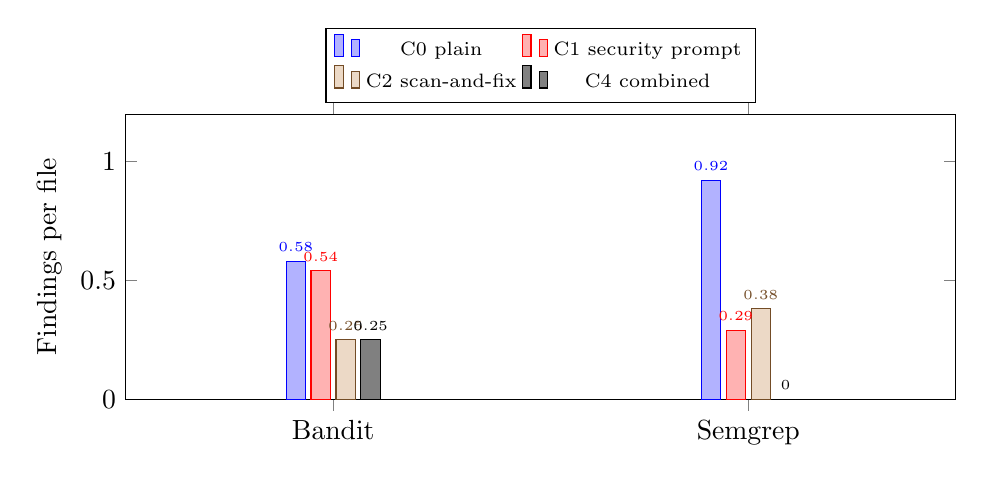
\begin{tikzpicture}
\begin{axis}[
  ybar, width=\columnwidth, height=5.2cm, bar width=7pt,
  symbolic x coords={Bandit,Semgrep}, xtick=data,
  ylabel={Findings per file}, ymin=0, ymax=1.2,
  enlarge x limits=0.5,
  legend style={at={(0.5,1.04)},anchor=south,legend columns=2,font=\scriptsize},
  nodes near coords,
  every node near coord/.append style={font=\tiny,/pgf/number format/fixed,/pgf/number format/precision=2}
]
\addplot coordinates {(Bandit,0.58) (Semgrep,0.92)};
\addplot coordinates {(Bandit,0.54) (Semgrep,0.29)};
\addplot coordinates {(Bandit,0.25) (Semgrep,0.38)};
\addplot coordinates {(Bandit,0.25) (Semgrep,0.00)};
\legend{C0 plain, C1 security prompt, C2 scan-and-fix, C4 combined}
\end{axis}
\end{tikzpicture}
\caption{Findings per file by condition (tasks 1--8, cleaned view).}
\label{fig:main}
\end{figure}

On Bandit, scan-and-fix cuts findings per file from 0.58 to 0.25, while the security prompt barely changes them (0.54). On Semgrep, the security prompt cuts findings from 0.92 to 0.29 and scan-and-fix reaches 0.38. Each mitigation therefore helps most on a different scanner. Combining them (C4) gave the lowest counts on both: 0.25 Bandit findings per file and no Semgrep findings at all in 24 files. Two cautions apply. Sixteen of the 24 C4 files were identical to their C1 versions because the scanners found nothing to fix, so the improvement comes from the eight files that were sent back to the model. And a loop that feeds scanner findings back optimises for the scanner's own rules, so a zero count shows that those rules no longer fire, not that the code is free of vulnerabilities. The medium-or-high percentages are tiny for Bandit (zero to two files out of 24), so they should not be over-read. With all rules enabled, the same eight tasks give Bandit 1.38, 0.54, and 0.25 findings per file and Semgrep 3.79, 1.79, and 2.67 for C0, C1, and C2. The higher all-rules Semgrep figure for C2 mostly reflects \texttt{render-template-string}, which was excluded from the C2 prompts and therefore left alone by the models.

\subsection{Plain Versus Security Prompt on All 16 Tasks}
Table~\ref{tab:sixteen} compares C0 and C1 on all 16 tasks (48 files per condition). With all rules enabled, the security prompt appears to be a strong intervention: Bandit's per-file count falls from 1.06 to 0.48 and the share of files with a medium or high Bandit finding falls from 58.3\% to 6.2\%. In the paired comparison, C1 has fewer Bandit findings than C0 in 28 of 48 model-task cases, equal in 13, and more in 7.

That result is almost entirely one setting. Flask debug mode (Bandit B201, CWE-94) accounts for 28 of C0's Bandit findings and zero of C1's. Once it is excluded, Bandit shows no difference at all (0.48 findings per file in both conditions), and the paired comparison becomes 12 fewer, 27 equal, and 9 more. Under Semgrep, the all-rules view shows a modest drop (2.44 to 1.69 per file) with no change in the share of files with a medium or high finding (66.7\% in both); the cleaned view shows a larger drop (0.52 to 0.21 per file, and 25.0\% to 14.6\% of files with a medium or high finding), with C1 fewer in 11 cases, equal in 32, and more in 5.

\begin{table}[t]
\caption{Plain (C0) versus security prompt (C1), all 16 tasks, three models, 48 files each}
\label{tab:sixteen}
\centering
\footnotesize
\begin{tabular}{@{}llrrr@{}}
\toprule
View & Metric & C0 & C1 & C1 fewer/eq/more \\
\midrule
All rules & Bandit per file & 1.06 & 0.48 & 28 / 13 / 7 \\
 & Bandit \% med+high & 58.3 & 6.2 & \\
 & Semgrep per file & 2.44 & 1.69 & 21 / 16 / 11 \\
 & Semgrep \% med+high & 66.7 & 66.7 & \\
\midrule
Cleaned & Bandit per file & 0.48 & 0.48 & 12 / 27 / 9 \\
 & Bandit \% med+high & 2.1 & 6.2 & \\
 & Semgrep per file & 0.52 & 0.21 & 11 / 32 / 5 \\
 & Semgrep \% med+high & 25.0 & 14.6 & \\
\bottomrule
\end{tabular}
\end{table}

\subsection{Differences Across Assistants (RQ4)}
Table~\ref{tab:models} gives the cleaned per-model results on all 16 tasks. Behaviour differs more across assistants than across workflows. Gemini's C1 code produced no Semgrep findings in 16 files (versus 0.62 per file for C0), and Copilot's Semgrep count fell from 0.69 to 0.31. Claude, by contrast, started with the lowest plain-prompt counts on both scanners and did not improve: its Bandit count rose from 0.31 to 0.62 per file with the security prompt, and its Semgrep count was essentially flat (0.25 to 0.31). A plausible reading is that the assistant with the cleanest baseline has the least to gain, but with 16 files per cell we cannot separate this from chance.

\begin{table}[t]
\caption{Findings per file by assistant, C0 $\rightarrow$ C1, all 16 tasks, cleaned view}
\label{tab:models}
\centering
\footnotesize
\begin{tabular}{@{}lrr@{}}
\toprule
Assistant & Bandit & Semgrep \\
\midrule
Claude & 0.31 $\rightarrow$ 0.62 & 0.25 $\rightarrow$ 0.31 \\
Copilot & 0.62 $\rightarrow$ 0.38 & 0.69 $\rightarrow$ 0.31 \\
Gemini & 0.50 $\rightarrow$ 0.44 & 0.62 $\rightarrow$ 0.00 \\
\bottomrule
\end{tabular}
\end{table}

On the eight tasks that also have C2, scan-and-fix reduced Bandit findings per file for Claude (0.25 to 0.25, unchanged from an already low baseline), Copilot (0.75 to 0.50), and Gemini (0.75 to 0.00), and Semgrep findings for Claude (0.38 to 0.12), Copilot (1.25 to 0.75), and Gemini (1.12 to 0.25).

\subsection{Which Weaknesses Change (RQ1, RQ2)}
In the cleaned Bandit view, the dominant C0 categories are hardcoded-password strings (CWE-259, 14 findings) and shell command execution (CWE-78, 7); the security prompt reduces them to 9 and 6, and introduces three SQL-related findings (CWE-89) that did not appear in C0. In the cleaned Semgrep view, the C0 findings are open redirects (CWE-601, 11), weak password requirements (CWE-521, 4), request forgery (CWE-918, 3), and cross-site scripting (CWE-79, 3). Under C1, open redirects fall to 1, and CWE-521 and CWE-79 disappear. Manual validation (Section~V-E) tempers this reading: all three sampled open-redirect findings were false alarms, and the hardcoded-string findings that remain under C1 were false alarms too. The cleaner conclusion is that the security prompt moves the code away from patterns the scanners flag, which for hardcoded secrets reflects a real improvement and for redirects mostly does not.

\begin{table}[t]
\caption{Findings by weakness (CWE), C0 $\rightarrow$ C1, all 16 tasks, cleaned view (48 files per condition)}
\label{tab:cwe}
\centering
\footnotesize
\begin{tabular}{@{}llr@{}}
\toprule
Tool & Weakness (CWE) & C0 $\rightarrow$ C1 \\
\midrule
Bandit & Hardcoded password string (259) & 14 $\rightarrow$ 9 \\
Bandit & OS command execution (78) & 7 $\rightarrow$ 6 \\
Bandit & SQL injection pattern (89) & 0 $\rightarrow$ 3 \\
Semgrep & Open redirect (601) & 11 $\rightarrow$ 1 \\
Semgrep & Weak password requirements (521) & 4 $\rightarrow$ 0 \\
Semgrep & Server-side request forgery (918) & 3 $\rightarrow$ 1 \\
Semgrep & Cross-site scripting (79) & 3 $\rightarrow$ 0 \\
Semgrep & Uncontrolled resource use (673) & 3 $\rightarrow$ 1 \\
\bottomrule
\end{tabular}
\end{table}

\subsection{Manual Validation of Findings}
Scanner output is not ground truth. We drew a random sample of 25 findings from the cleaned view across tools, models, and conditions (14 from C0, 8 from C1, and 3 from C2) and judged each flagged line from the surrounding code. Of the 25, 8 were real weaknesses, 14 were false alarms, and 3 were unclear, so the estimated false-positive rate is 56\% (64\% if the unclear cases are set aside). The labels come from a single reviewer and were not cross-checked.

The pattern by rule is informative. All five sampled hardcoded-secret findings in C0 were real: a literal \texttt{secret\_key} or login password in the source. Both sampled hardcoded-password findings in C1 were false alarms (a hash-method name, ``scrypt'', and a deliberately wrong password in a test routine), so the security prompt appears to have removed real hardcoded secrets while leaving string constants that merely look like them. All three open-redirect findings were false alarms: two redirect back to the current page, and one passes the target through a sanitising helper. Both informational \texttt{import subprocess} findings and both \texttt{assert} findings were also false alarms. The remaining real findings were an unvalidated host argument passed to \texttt{ping} (task 8, C0) and two servers bound to all network interfaces. The sample is small, so these rates are rough, but they show that finding counts overstate the number of real vulnerabilities.

\subsection{Does the Code Still Run? (RQ3)}
A full functional test of 120 programs was beyond our time budget, so we ran a minimal smoke test. Each file was imported as a Flask application in its own process and temporary folder, with dummy values set for the environment variables that secure code requires (secret keys and API keys), and the home page was requested (\texttt{GET /}). A status code below 500 counted as working. Thirty-three of the 144 files define no web application (for example the ping, serialization, and encryption tasks), leaving 111 applications.

Table~\ref{tab:smoke} shows the results. Working rates were similar across conditions: 28 of 35 applications under C0, 27 of 34 under C1, 18 of 21 under C2, and 18 of 21 under C4. The security prompt and the fix loops therefore did not noticeably reduce the share of applications that start. The failures were of different kinds. Four files failed to import: two Copilot C1 files (tasks 9 and 13) had syntax errors, and two (one C1, one C4) required environment variables we had not set (\texttt{ADMIN\_EMAIL} and \texttt{PUBLIC\_BASE\_URL}), another example of secure code refusing to start without configuration. Ten applications returned HTTP 500 on the home page; five of them were the comment-board task (task 11) across models, which probably needs database setup or a form token that our harness does not provide, though we did not investigate. Five files could not be tested because they need packages we did not install (for example a mail or rate-limiting extension, or Django), and one hung. A request to the home page is a weak test: it shows that an application starts and serves a page, not that its logic is correct, and a ``fix'' that quietly removes functionality would not be caught. Behavioural testing remains the main gap for RQ3.

\begin{table}[t]
\caption{Smoke test: applications by outcome (33 of 144 files define no web app and are excluded)}
\label{tab:smoke}
\centering
\footnotesize
\begin{tabular}{@{}lrrrrr@{}}
\toprule
Cond. & Apps & Works & HTTP 500 & Import err. & Other \\
\midrule
C0 & 35 & 28 & 5 & 0 & 2 \\
C1 & 34 & 27 & 3 & 3 & 1 \\
C2 & 21 & 18 & 1 & 0 & 2 \\
C4 & 21 & 18 & 1 & 1 & 1 \\
\bottomrule
\end{tabular}
\end{table}

\subsection{Threats to Validity}
\textbf{Scanner dependence.} Findings are not confirmed vulnerabilities. Static analyzers miss logic and authorisation flaws, and they raise false alarms, so improvements in counts may not equal improvements in security. \textbf{Noisy-rule choices.} Our cleaned view depends on four exclusions we made after seeing the data. We therefore report both views, but the choice is a judgment. \textbf{Small sample.} Most cells contain 8 to 24 files and findings are single digits, so we avoid significance claims. \textbf{Interface and version drift.} We used free chat interfaces, partly by hand, with unpinned model versions. \textbf{Prompt design.} The security sentence is one phrasing; other phrasings may behave differently. \textbf{Task scope.} All tasks are small Flask programs; larger projects, other languages, and agentic assistants may differ. \textbf{C2 scope and design.} C2 covers eight tasks, and one noisy rule was withheld from the fix prompts, which affects the all-rules comparison. C4 covers the same eight tasks; most of its files were unchanged copies of C1, and a fix loop optimises for scanner rules.

\section{Discussion, Lessons Learned, and Future Work}
\subsection{Answers to the Research Questions}
\textbf{RQ1 (baseline).} Plain-prompt code averaged 1.06 Bandit and 2.44 Semgrep findings per file with all rules enabled (0.48 and 0.52 in the cleaned view). The dominant categories were Flask debug mode, hardcoded-password strings, shell command execution, and open redirects.

\textbf{RQ2 (mitigations).} The security prompt reliably removed debug mode and several Semgrep categories, but left Bandit's cleaned count unchanged. Scan-and-fix (C2) lowered Bandit's count to 0.25 per file. In effort terms, C1 costs one added sentence per prompt, while C2 costs a scan and one extra chat per file that has findings (23 of 24 files in our run). C4, the combination, gave the lowest counts on both scanners and needed an extra chat for only 8 of 24 files, because the security prompt had already removed most findings.

\textbf{RQ3 (functionality).} In a minimal smoke test, 28 of 35 (C0), 27 of 34 (C1), and 18 of 21 (C2), and 18 of 21 (C4) applications started and served their home page, so the mitigations did not noticeably reduce the share that run. Two Copilot C1 files had syntax errors. Behavioural correctness was not tested, so this question is only partly answered.

\textbf{RQ4 (assistants).} Yes: Gemini and Copilot improved under the security prompt, while Claude, which started cleanest, did not. With 16 files per cell we cannot rule out chance.

\subsection{Lessons Learned}
\textbf{Headline numbers can hide one setting.} With all rules enabled, the security prompt looked decisive. A single misconfiguration explained most of it. Reporting results with and without such items is essential, and the single-setting finding is itself useful: the security sentence reliably stops assistants from leaving Flask's debug server on.

\textbf{Scanners can penalise safer code.} Claude's explicit \texttt{TESTING=False}, written in response to ``set safe defaults,'' triggered a hardcoded-configuration rule. Prompts that make code more explicit can therefore raise scanner counts without making it less secure.

\textbf{Counts overstate real risk.} In our validation sample, 14 of 25 findings were false alarms, including every sampled open-redirect finding, so a reduction in counts should be read as a reduction in flagged patterns, not necessarily in vulnerabilities.

\textbf{Mitigations are complementary, not interchangeable.} Scan-and-fix works on whatever the scanner can detect, so it was strongest on Bandit's categories. The security sentence addresses general habits (redirects, password policy, output encoding) that Semgrep's rules cover. The combined workflow (C4) did best on both scanners: the prompt prevents common mistakes up front, and the scan-and-fix loop cleans up what the scanner can still see.

\textbf{Scan-and-fix can also teach suppression.} One C2 output added \texttt{\# nosec} comments next to the flagged lines. Disabling suppression when scanning is a cheap safeguard for any evaluation of feedback loops.

\textbf{Practical guidance.} For a developer who will not review the code in depth, adding a one-line security instruction is nearly free and removes a dangerous default, but it is not a substitute for scanning; running a scanner and asking the model to fix the result is a second, separate improvement.

\subsection{Future Work}
Run C3 (cross-model review); expand to more tasks and samples per prompt so that confidence intervals are possible; add dynamic testing and functional tests so that RQ3 can be answered properly; evaluate agentic coding assistants that run and test their own code; pin model versions through APIs; and add confirmed-vulnerability labels, for example through formal verification as in FormAI~\cite{tihanyi2023formai}, to complement scanner counts.

\section{Conclusion}
We compared four developer-level workflows for generating Flask applications with free AI assistants: a plain prompt, a one-sentence security prompt, a scan-and-fix loop, and the last two combined. Raw scanner totals suggest that a security prompt removes most severe findings, but most of that effect is one setting, Flask debug mode. After removing four noisy rules, the security prompt lowers Semgrep findings (0.52 to 0.21 per file) without changing Bandit's (0.48 per file), scan-and-fix lowers Bandit findings (0.58 to 0.25 on the same tasks), the two combined give the lowest counts on both scanners (0.25 and 0.00 per file, with only eight files needing a fix), and results differ across assistants. The measurements are scanner-based, the sample is small, and functional testing is incomplete, so the findings should be read as patterns that motivate larger studies. The main methodological lesson is to inspect which rules drive a result before trusting a headline number.

\section*{Availability}
The task prompts, generated programs, and analysis scripts are available from the author at \url{https://github.com/hephz-pekun/vibe-code-security-study}.

\begin{thebibliography}{00}
\bibitem{pearce2022asleep} H. Pearce, B. Ahmad, B. Tan, B. Dolan-Gavitt, and R. Karri, ``Asleep at the keyboard? Assessing the security of GitHub Copilot's code contributions,'' in \emph{Proc. IEEE Symp. Security and Privacy (SP)}, 2022. [Online]. Available: arXiv:2108.09293.
\bibitem{perry2023users} N. Perry, M. Srivastava, D. Kumar, and D. Boneh, ``Do users write more insecure code with AI assistants?'' in \emph{Proc. ACM SIGSAC Conf. Computer and Communications Security (CCS '23)}, Copenhagen, Denmark, Nov. 2023, pp. 2785--2799, doi: 10.1145/3576915.3623157.
\bibitem{tihanyi2023formai} N. Tihanyi et al., ``The FormAI dataset: Generative AI in software security through the lens of formal verification,'' in \emph{Proc. 19th Int. Conf. Predictive Models and Data Analytics in Software Engineering (PROMISE '23)}, San Francisco, CA, USA, Dec. 2023, doi: 10.1145/3617555.3617874.
\bibitem{chen2021codex} M. Chen et al., ``Evaluating large language models trained on code,'' arXiv:2107.03374, 2021.
\bibitem{khoury2023secure} R. Khoury, A. R. Avila, J. Brunelle, and B. M. Camara, ``How secure is code generated by ChatGPT?'' in \emph{Proc. IEEE Int. Conf. Systems, Man, and Cybernetics (SMC)}, 2023, arXiv:2304.09655.
\bibitem{fu2023security} Y. Fu et al., ``Security weaknesses of Copilot generated code in GitHub,'' arXiv:2310.02059, 2023. % TODO verify
\bibitem{sandoval2023lost} G. Sandoval, H. Pearce, T. Nys, R. Karri, S. Garg, and B. Dolan-Gavitt, ``Lost at C: A user study on the security implications of large language model code assistants,'' in \emph{Proc. USENIX Security Symp.}, 2023.
\bibitem{pearce2023repair} H. Pearce, B. Tan, B. Ahmad, R. Karri, and B. Dolan-Gavitt, ``Examining zero-shot vulnerability repair with large language models,'' in \emph{Proc. IEEE Symp. Security and Privacy (SP)}, 2023.
\bibitem{he2023hardening} J. He and M. Vechev, ``Large language models for code: Security hardening and adversarial testing,'' in \emph{Proc. ACM SIGSAC Conf. Computer and Communications Security (CCS '23)}, 2023.
\bibitem{tony2023llmseceval} C. Tony, M. Mutas, N. E. D. Ferreyra, and R. Scandariato, ``LLMSecEval: A dataset of natural language prompts for security evaluations,'' in \emph{Proc. IEEE/ACM Int. Conf. Mining Software Repositories (MSR)}, 2023.
\bibitem{bhatt2023cyberseceval} M. Bhatt et al., ``Purple Llama CyberSecEval: A secure coding benchmark for language models,'' arXiv:2312.04724, 2023.
\bibitem{madaan2023selfrefine} A. Madaan et al., ``Self-Refine: Iterative refinement with self-feedback,'' in \emph{Proc. Advances in Neural Information Processing Systems (NeurIPS)}, 2023.
\bibitem{owasp} OWASP Foundation, ``OWASP Top Ten.'' [Online]. Available: https://owasp.org/www-project-top-ten/ Accessed: Nov. 19, 2026.
\bibitem{cwe} MITRE Corporation, ``Common Weakness Enumeration (CWE).'' [Online]. Available: https://cwe.mitre.org/ Accessed: Nov. 19, 2026.
\bibitem{bandit} PyCQA, ``Bandit: Security linter for Python,'' v1.9.4. [Online]. Available: https://github.com/PyCQA/bandit Accessed: Nov. 19, 2026.
\bibitem{semgrep} Semgrep, Inc., ``Semgrep,'' v1.185.0. [Online]. Available: https://semgrep.dev Accessed: Nov. 19, 2026.
\end{thebibliography}

\end{document}